% Copyright (c) 2014,2016 Casper Ti. Vector
% Public domain.

\chapter{PKI}

本章将对PKI系统进行详细介绍,首先从系统架构对PKI进行解析,阐述系统中包含的角色和各自的功能;其后将对证书进行介绍,包括证书的结构以及证书的生命周期;最后对本系统存在的问题以及相应的解决方案进行简要叙述。

\section{PKI系统}

公钥基础设施PKI(Public Key Infrastructure)作为一种遵循标准的密码管理平台,其可以为网络应用提供密钥和证书管理服务,使用户可以在多种应用环境下方便的使用加密和数字签名技术,从而保证数据的机密性、完整性、有效性和抗抵赖性。

本小节将从框架和其包含的相关组件对PKI进行介绍。

\subsection{PKI基本框架}

PKI框架中包括安全和操作策略,安全服务以及支持公钥密钥和证书管理的交互式协议。公钥和对应证书的生成、分发和管理将通过授权机构(CAs)、注册机构(RAs)和目录服务来完成\supercite{weise2001public},它们将会建立等级信任或者说信任链。以上提到CAs、RAs和目录服务可以将数字证书用于鉴定不同实体的身份,而PKI拥有如此架构的目的是为了能支持并完成数据、凭证在各种不安全环境下的安全交换。

\subsection{PKI的系统构成}

在PKI系统可能会包含一下组成部分:

\begin{itemize}
	\item 

	注册机构(RA)

	RA的作用是执行身份验证和处理新的数字证书请求、更新数字证书请求和吊销数字证书请求。

	\item

	授权机构(CA)

	CA将创建和发布数字证书以及证书吊销列表(CRLs),其颁发的数字证书将对主体名称(如用户表示)和绑定的公钥进行签名。

	\item

	验证结构(VA)

	VA是一个PKI的管理实体,可以用来检查数字证书的有效性。当证书的签发者和证书的状态管理服务有不同的服务提供者提供时,将使用到VA。

	\item

	用户

	PKI面对的用户是证书持有者或者密钥持有者,通过遵从认证运作规范(CPS)和证书策略(CP)获得证书,完成证书和密钥对的绑定。PKI系统中的用户可以是个体、组织或者非个人实体,有责任保存好自己的私钥不被泄露。

	\item

	依赖方

	依赖方在PKI系统中接收、验证和接受数字证书。

	\item

	证书策略(CP)

	证书策略是一组安全规则要求,适用于一类应用系统的共同安全需求。

	\item

	认证运作规范(CPS)

	CPS描述了CA提供数字证书服务的规则和处理方式,其中可能会包括提供服务描述,证书生命周期的管理细则、业务信息、法律义务和金融责任等。
\end{itemize}

图\ref{fig:pki}将给出以上所提到组件之间的关系,图中的剪头将表示数字证书和证书状态信息的传递。

\begin{figure}[htbp]
 	\centering
 	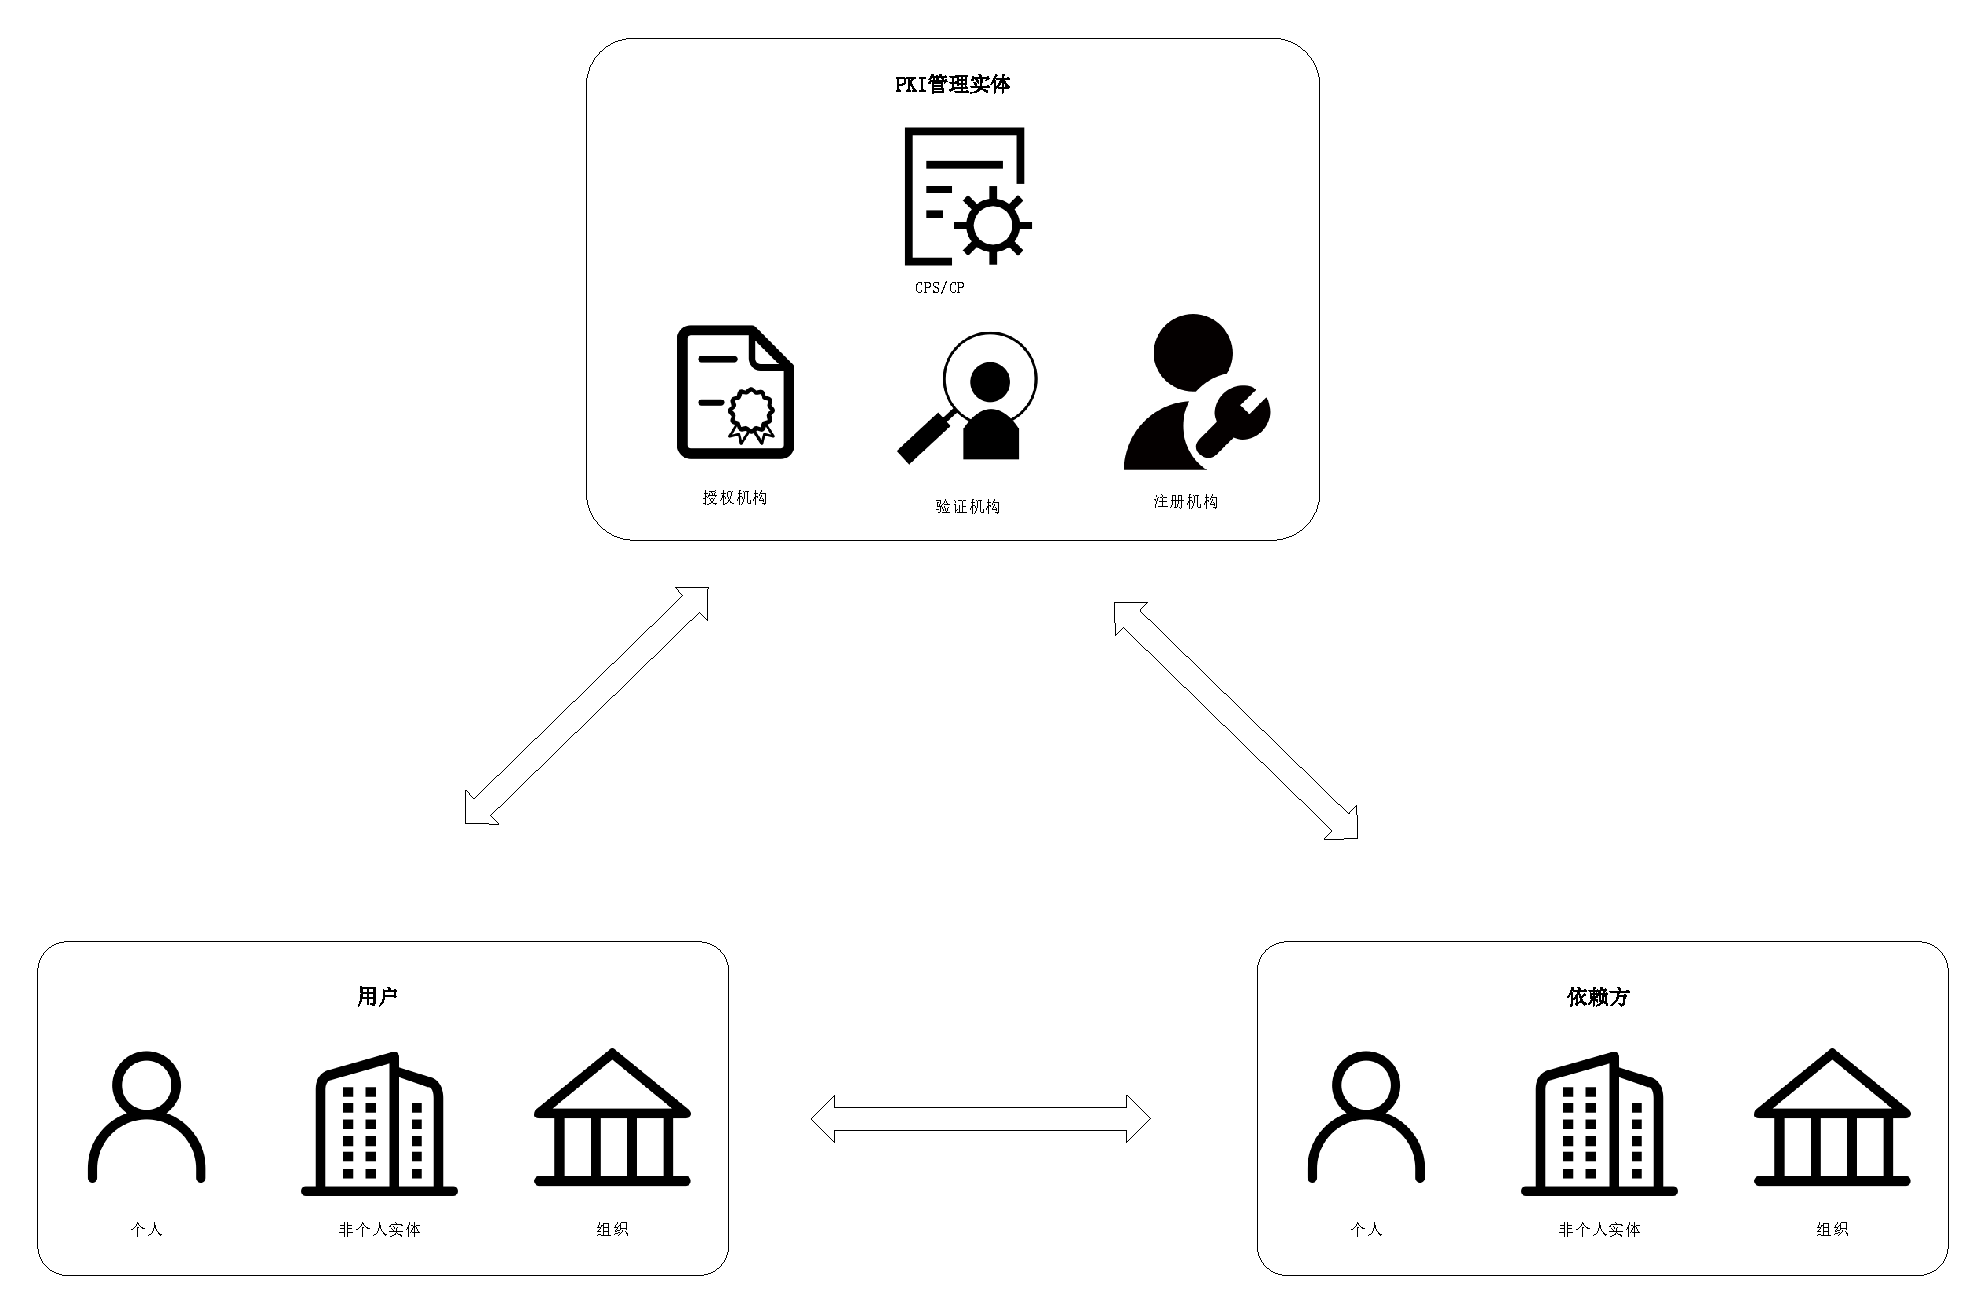
\includegraphics[width = 0.8\textwidth]{img/pki}
 	\caption{PKI组成部分}\label{fig:pki}
\end{figure}


\subsection{证书的生命周期}

证书作为包含公钥、数字签名以及一些其它附带信息的数字文档,在PKI系统中充当着公钥交换、存储和使用的介质。了解证书的申请、签发和使用,可以明白PKI系统的是如何运作,并从中发现可能存在的问题。

证书的声明周期从用户提交准备的证书签发请求(CSR)并提交给其选择的CA开始。CSR中包含了用户的公钥和相应的信息,并通过签名的方式表明对相应私钥的所有权。同时,CSR可以携带额外的信息元,但在实际使用过程中并没有全部使用。CA可以对CSR中的内容进行重写,放置一些其它的信息在证书中。

其后CA通过遵循验证流程,对用户进行身份验证。待成功完成验证之后,CA将签发证书,同时提供验证至更证书的所有中间证书。

得到证书后,用户就可以再证书过期之前使用证书。如果证书对应的私钥泄露,证书将可以被吊销,该过程和证书签发的过程类似。


[图]

\section{系统中存在的问题}

\section{已有的改善措施}

% vim:ts=4:sw=4
